\section{Open calculations}\label{sec:22.1}

The phonon-assisted loss function of silicon is specified down to its grids, its Wannier manifold and its tolerances, and its plane-wave stages cost some 350 to 450 core-hours (\cref{app:E.14}). Done, it would turn the estimate of the silicon window into a number with an error bar. Most open calculations of the book are of this kind: specified in \crefrange{chap:30}{chap:32}, and each tied to a definite result. They differ in what they would move, from the reach of the running example to a correction of a few percent on a special target, and in the test that separates a correct result from a converged one. The dark-matter masses quoted below are in MeV; a mass $\mchi$ can deposit at most $\mchi v_{\mathrm{max}}^2/2$, with $v_{\mathrm{max}} = 2.65\times10^{-3}$ the largest dark-matter speed in the laboratory (\cref{sec:1.2}), so \SI{0.333}{MeV} deposits at most \SI{1.17}{eV}.

\subsection{Sum rules and controls}\label{sec:22.1-checks}

An exact relation holds for every Hamiltonian of a stated class. A result that violates it has an error in its sum over states, in its labeling of final states or in its normalization, whatever it approximates in the interactions. A control compares the result with a measurement that the calculation was not fitted to. The first kind tests completeness and bookkeeping, the second tests the physics, and an open calculation needs both. Exact relations have a limit of their own: an approximation that does not conserve particle number at its vertices violates them by itself, as the bare BCS bubble does (\cref{sec:7.2}), and its error then has to be read from a conserving version of the same response.

The exact relations of the book are the $f$-sum rule and its shares among the sectors of \cref{sec:8.6} (\cref{eq:4.3-fsum,eq:8.6-fsum-e,eq:8.6-fsum-k,eq:8.6-fsum-ek}) and its transfer between zero-phonon lines and sideband (\cref{eq:13.7-fsum}); positivity of $S_{ab}$ and Kramers--Kronig (\cref{eq:4.2-positivity,eq:4.3-KK}); the translation Ward identity with its soft and boost limits (\cref{eq:8.3-ward,eq:8.3-soft,eq:8.3-boostward}); the zeros that symmetry imposes; and the conservation laws of the cascade and of detector transport (\cref{eq:D.43-moments,eq:20.1-hecht,eq:20.1-work}). Three of them carry an instruction for a calculation. A table that stores $S_{ab}$ with a negative eigenvalue, or a real part that fails the transform, fails before any comparison with data. The acoustic sum rule \cref{eq:5.2-asr} is imposed on the dynamical matrix, never by setting the electron--phonon vertex to zero at small phonon momentum (\cref{app:E.14}). And a calculation that returns the symmetry zeros at the level of its numerical noise has its phases and labels right: the interference (Fano) term between a zero-phonon state and the phonon-assisted continuum, which vanishes at the level of one-body self-energies in crystals invariant under inversion combined with time reversal (\cref{sec:8.6}), the paths that the glide rule \cref{eq:13.9-glide} removes on the valley axis of silicon, and the $\ell = 2$ component of any scalar response of a cubic crystal. The controls are measured absorption for a finite-$q$ response in its optical limit, neutron data for computed phonons, the measured pair energy and Fano factor of silicon for a cascade, and the neutron-calibrated charge yields of silicon and germanium. \Cref{tab:22-calc} gives the relation and the control that each calculation must pass.

\subsection{Priority list of calculations}\label{sec:22.1-list}

\Cref{tab:22-calc} lists, each once, the open calculations that would change a printed result, limit or ranking of the book, in the order of the results they change; the other calculation steps appear among the gaps of \cref{tab:22-gaps}. A calculation that serves several sections appears in the row of its largest effect, with the others named. The order starts with the silicon electron recoil, the running example and the channel on which most published limits rest.

{\scriptsize\setlength{\tabcolsep}{3pt}\setlength{\LTcapwidth}{\linewidth}
\begin{longtable}{@{}>{\raggedright\arraybackslash}p{0.25\linewidth}>{\raggedright\arraybackslash}p{0.305\linewidth}>{\raggedright\arraybackslash}p{0.305\linewidth}>{\raggedright\arraybackslash}p{0.09\linewidth}@{}}
  \caption{Open calculations that would change a printed result, limit or ranking of the book, ordered by the result each would change; the remaining calculation steps are in \cref{tab:22-gaps}. Calculation: what is to be computed, with the section that specifies it. Result: the number or statement of the book that the calculation replaces, with its present size; masses are dark-matter masses. Check: the exact relation (sum rule, positivity, symmetry zero, conservation law) and the control against data that the result must pass. Section: where the item is stated. The guide is the ranking of crystals by figure of merit in \cref{sec:21.7}, its survivors are the eleven crystals with a documented detector record, and $P(\mathrm{first})$ is the probability that a crystal ranks first in a row of the guide.}
  \label{tab:22-calc}\\
  \toprule
  Calculation & Result it changes & Check it must pass & Section \\
  \midrule
  \endfirsthead
  \toprule
  Calculation & Result it changes & Check it must pass & Section \\
  \midrule
  \endhead
  \bottomrule
  \endfoot
  \multicolumn{4}{@{}l}{\emph{Silicon electron recoil}} \\
  Phonon-assisted loss function from the four-path amplitude, with the zero-phonon rate on common bins (\cref{app:E.14}) & rate and reach from the onset at \SI{0.333}{MeV} to the first zero-phonon edge at \SI{0.405}{MeV}, now an estimate normalized to the measured cold edge; mass up to which the phonon-assisted rate leads (about \SI{0.43}{MeV}, at least \SI{0.42}{MeV}); band of comparable rates up to \SI{0.51}{MeV} & optical limit against the measured \SI{20}{K} edge; zero rate at $g = 0$; frozen phonon at X; soft acoustic limit \cref{eq:8.3-soft}; symmetry zeros on the valley axis; band-sum $f$-sum with the nonlocal part separated (\cref{we:22-fsum}); transfer rule \cref{eq:13.7-fsum} & \cref{sec:13.9} \\
  Transverse-acoustic frequency $\omega_{\mathrm{TA}}(\vect{Q}^*)$ by direct DFPT at two lattice constants and with a second pseudopotential (\cref{app:E.14}) & onset 0.3332 and \SI{0.3374}{MeV}; 0.3336 and \SI{0.3378}{MeV} with the branch scaled to neutron data & direct values bracket the interpolated one within \SI{0.3}{meV}; transverse-acoustic branch against neutron data & \cref{sec:13.9} \\
  Pair channel at finite $q$ in a supercell with local fields (\cref{app:E.16}) & screening correction 0.3 to 2.6 relative to the optical calibration; pair-channel residual unsized & reduces at $q \to 0$ to the optical calibration, which contains the pair channel & \cref{sec:13.4} \\
  Finite-momentum Bethe--Salpeter response of silicon and germanium with the coupling block, bound lines added from computed masses and vertices (\cref{app:E.15}) & attraction, $\times1.28$ on the rate from 3.6 to \SI{10}{MeV} (heavy mediator), \SI{39}{\percent} of the variance of the one-standard-deviation factor 1.48 at \SI{3}{MeV}, \SI{93}{\percent} together with the converged table of the next row; triplet channel; spin--orbit mixing at the germanium edge & $f$-sum \cref{eq:4.3-fsum} to a percent; measured optical $\varepsilon_2$ at $q \to 0$; coupling block against its estimate of \SI{10}{\percent} & \cref{sec:10.5,sec:10.10} \\
  One converged independent-particle table, and all-electron random-phase response with local fields to \SI{10}{keV} with the current and kinetic rows as external rows (\cref{app:E.6,app:E.16}) & tabulation spread, $\times3.2$ at \SI{1}{MeV} and $\times1.34$ at \SI{3}{MeV}; local fields above $2q_0$, $\times1.24$ at \SI{10}{MeV}; velocity couplings, now at least 16 times the static-electron formula & $f$-sum at small $q$, where the published tables give 1.1--1.2 against 0.93 at 0.3--$0.7\,q_0$, and at \SI{10}{keV}; positivity of $S_{ab}$; Kramers--Kronig & \cref{sec:10.1,sec:10.2,sec:10.4} \\
  Crystal final states of the germanium $3d$ shell; four-component response (\cref{app:E.15}) & $3d$ share near \SI{30}{MeV}: $3d$/valence between 0.07 and 0.69 & relativistic $f$-sum shift, $-\SI{0.76}{\percent}$ & \cref{sec:10.6} \\
  \midrule
  \multicolumn{4}{@{}l}{\emph{Germanium window}} \\
  Quasiparticle bands of germanium with spin--orbit coupling; transverse-acoustic phonons on a $6^3$ grid (\cref{app:E.14}) & zero-phonon edge, not known: \SI{0.32}{MeV} in an on-axis parabolic estimate that orients but does not bound it (\cref{sec:13.1}), above the phonon-assisted onset 0.2119--\SI{0.2141}{MeV}; germanium electronic window and crossovers of \cref{sec:17.1} & valley order, L below $\mathrm{\Gamma}$; both gaps within \SI{0.1}{eV} of the measured 0.744 and \SI{0.89}{eV}; transverse mass at L within $0.010\,m_e$ of $0.0815\,m_e$ and mass at $\mathrm{\Gamma}$ within $0.005\,m_e$ of $0.038\,m_e$; transverse-acoustic branch at X and L against neutron data & \cref{sec:13.9,sec:17.1} \\
  \midrule
  \multicolumn{4}{@{}l}{\emph{Migdal rate and ranking}} \\
  Coherent zero-phonon Migdal response of silicon from \SI{0.75}{keV} to $2q_{\mathrm{BZ}}$, all cross-site terms and local fields (\cref{app:E.18}) & nearly all of the silicon Migdal rate up to \SI{1}{MeV}, \SI{33}{\percent} at 2 and \SI{7}{\percent} at \SI{3}{MeV}, now unsized & boost limit \cref{eq:8.3-boostward} as $q \to 0$ (the diagonal form is 14.9 times too high there); diagonal form above $2q_{\mathrm{BZ}}$; partial sum rule \cref{eq:8.6-fsum-k} & \cref{sec:12.4,sec:17.1} \\
  Off-diagonal $\varepsilon^{-1}_{\vect{G}\vect{G}'}$ in the Migdal rate, with an all-electron or PAW ion vertex and a converged $\vect{G}$ sum (\cref{app:E.18}) & factor 1.2--1.4 from a model whose lower end is not bounded & diagonal local fields, $\times1.35$ (\cref{lim:12.3a}); plain $1/\varepsilon_{00}$ & \cref{sec:12.3} \\
  $\vect{Q}$-resolved drag mass $\delta M_{\kappa\kappa}(\vect{Q})$ of crystalline silicon; ratio of the self-consistent to the rigid Wannier amplitude (\cref{app:E.18}) & on-site drag mass $\delta M_{II}$, valence part $18.6\,m_e$ bounded to 12--$24\,m_e$ (the trace value $14\,m_e$ is exact but is not the on-site element); Wannier picture bounded by 1.6, 0.54 and 0.25 at 20, 50 and \SI{100}{eV} & trace rule \cref{eq:12.5-trace}, $14\,m_e$ per atom at $\vect{Q} = 0$; acoustic sum rule; partial sum rule \cref{eq:8.6-fsum-k} & \cref{sec:12.3,sec:12.5} \\
  Loss function $L(\vect{k},\omega)$ near the gap, $|\vect{k}|$ up to a few keV, for every survivor (\cref{app:E.16}) & Migdal row of the guide, without a reading (largest $P(\mathrm{first})$ 0.315 among the survivors, 0.498 in the full pool) & inverse fourth moment against the partial $f$-sum bound from \cref{eq:17.5-partial}; gap of the ground state equal to the measured one & \cref{sec:17.5,sec:21.7} \\
  \midrule
  \multicolumn{4}{@{}l}{\emph{Charge of a nuclear recoil and the cascade}} \\
  Close-collision excitation kernel \cref{eq:19.2-kernel} for Si--Si and Ge--Ge collisions, with its exchange--correlation spread (\cref{app:E.23}) & charge yield below the binary thresholds, 352 and \SI{399}{eV}; measured silicon yield 0.10 at \SI{100}{eV} with no threshold, germanium $(25 \pm 3)\,\%$ at \SI{254}{eV}; probability of a recoil without charge & the measured yields and Fano factors of silicon and germanium & \cref{sec:19.2} \\
  Cascade without a fitted constant: impact ionization from the $GW$ self-energy, computed phonon couplings of both carriers, excitonic final states, converged photon seed; then germanium and GaAs with spin--orbit coupling (\cref{app:E.13,app:E.24}) & pair energy without a fitted constant, \SI{4.15}{eV} $[3.95, 4.73]$ with a class systematic of at least $\pm\SI{0.4}{eV}$; two-pair fraction at \SI{5}{eV}, 0.097 in $[0.030, 0.173]$; $F_{\mathrm{eh}} = 0.114$; photon against dark-matter seed & measured $\varepsilon_{\mathrm{eh}} = \SI{3.749}{eV}$ and $F_{\mathrm{eh}} = 0.119$ of silicon, \SI{2.96}{eV} of germanium at \SI{77}{K}; normalization, moments \cref{eq:D.43-moments}, one pair below $(1 + \theta_{\mathrm{ii}})\Eg$ & \cref{sec:18.3,sec:18.4} \\
  Pair energies of the crystals outside the validated range, and cascade tables $P_{\mathrm{casc}}$ for every survivor (\cref{app:E.13,app:E.24}) & threshold-in-quanta row of the guide: GaSb ranks ahead of germanium with probability 0.83, and the lead salts are not separated, on estimates with the conventional width 0.21 & measured pair energies of the validated range; one pair below $(1 + \theta_{\mathrm{ii}})\Eg$ in every table & \cref{sec:18.4,sec:21.7} \\
  Binding, trapping and capture rates of pairs at millikelvin in silicon and germanium (\cref{app:E.24}) & capture fraction (\SI{0.54}{\percent}, 0.32 to \SI{0.77}{\percent}, closes the silicon Fano gap); fraction of excitons never split; release law of the gap energy & measured bound-exciton Auger lifetime; the measured silicon Fano factor & \cref{sec:18.5,sec:20.5} \\
  \midrule
  \multicolumn{4}{@{}l}{\emph{Readout and delayed signals}} \\
  Collection kernels of a stated detector from validated phonon and charge transport (\cref{app:E.25}) & collection ratio, 0.81--1.02 in the mean-field estimate against the 1.128 that collection alone needs; stored-energy bound & Hecht relation, charge sum, bias work, Fano factor of the drifted charge; energy conservation of film phonons & \cref{sec:19.5,sec:20.5} \\
  Emission cross-sections of shallow and over-charged traps; Luke emission into both acoustic branches (\cref{app:E.25,app:E.12}) & delayed charge and space-charge field over an exposure; spectrum of Luke phonons & measured drift velocity against field; phonon signal at fixed field & \cref{sec:20.1} \\
  Release paths of close Frenkel pairs: tunneling exponent and $E_{\mathrm{reorg}}/\varepsilon^{\mathrm{hop}}$ to about \SI{5}{\percent} (\cref{app:E.22}) & delayed release of stored energy at millikelvin; bound on the low-energy excess & stored-energy sum rule \cref{eq:19.6-sumrule} & \cref{sec:19.6} \\
  \midrule
  \multicolumn{4}{@{}l}{\emph{Lattice, spin, superconducting and novel targets}} \\
  Anharmonic template of silicon from cubic and quartic force constants, anchored to a path-integral kinetic energy (\cref{app:E.19}) & few-phonon weights between $q_{\mathrm{BZ}}$ and about \SI{20}{keV} & exact moments with Hankel positivity \cref{eq:8.3-hankel}; kinetic energy within $\pm\SI{0.2}{\percent}$ & \cref{sec:11.5,sec:11.9} \\
  All-electron density response of displaced atoms above the zone (\cref{app:E.17}) & multiphonon rate of a charge coupling far above $q_{\mathrm{BZ}}$ & translation Ward identity \cref{eq:8.3-ward} & \cref{sec:11.3,sec:11.9} \\
  Zero-temperature two-phonon absorption of silicon below \SI{65}{meV}, from the derivatives of the Born charges (\cref{app:E.17}) & electromagnetic channel of vector absorption in the one-phonon band; the isotope channel now exceeds it at least $5.0\times10^3$ times at \SI{50}{meV} & the measured \SI{293}{K} absorption, reproduced at that temperature; the bound \cref{eq:11.6-Tbound} & \cref{sec:11.6} \\
  Cubic-harmonic components of the silicon loss function with local fields (\cref{app:E.16}) & electronic part of the daily modulation & $\ell = 2$ component zero; no first moment in the components with $\ell \ge 4$, since \cref{eq:4.3-fsum} is isotropic & \cref{sec:11.7} \\
  GaAs dynamical quadrupoles (\cref{app:E.5}); kinetic energy of the core electrons of free gallium and arsenic atoms & acoustic charge of the polar rate, at most \SI{3}{\percent}; GaAs scalar rate, $-\SI{19}{\percent}$ in a parametric estimate & small-$\vect{Q}$ angular dependence of the vertex; virial theorem of the free atom & \cref{sec:11.2,sec:11.8} \\
  Magnetic response of NiO beyond linear spin waves, with its anisotropy near the lightest masses (\cref{app:E.20}) & one-magnon weight, high by \SI{7.8}{\percent}; rate near the edge & total-spin sum rule (\cref{sec:14.1}) & \cref{sec:14.1} \\
  Two-magnon ladder \cref{eq:14.2-ladder} for NiO and YIG on $30^3$ to $40^3$ wavevectors (\cref{app:E.20}) & two-magnon continuum, about 0.04 of the NiO spin response moved in energy; existence of a bound pair below the continuum & sum rule of the ladder (weight moved, not added); total-spin sum rule & \cref{sec:14.2} \\
  Current response $\boldsymbol{\mathcal{G}}_{\mathrm{OA}}(\vect{q},\omega)$ of tellurium or $\alpha$-quartz at $\pm\vect{q}$, with spin--orbit coupling and the nonlocal current vertex (\cref{app:E.20}) & chiral response at keV momenta, now only the scale $q\,g_{33} = 0.034$ at \SI{1}{keV} in quartz & density-functional optical activity at small $q$; zero in silicon & \cref{sec:14.5} \\
  Disorder-averaged loss function of amorphous WSi at keV momenta and the distribution of its local gap (\cref{app:E.20}) & rate of an amorphous film, unsized; it differs from the rate of the averaged $\varepsilon$ at the order of the variance of $\varepsilon$ & computed conductivity against the measured resistivity & \cref{sec:15.3} \\
  Transport function $\alpha^2F_{\mathrm{tr}}$ of aluminum below a few meV (\cref{app:E.20}) & phonon-assisted absorption within a few meV of $2\Delta_{\mathrm{BCS}}$; the free-electron model holds $1.25\times10^4$ times too much weight there & acoustic sum rule of the vertex; $\lambda_{\mathrm{tr}}$ against the resistivity value 0.39 & \cref{sec:15.4} \\
  Superconducting phonon-assisted absorption with Eliashberg spectral functions, with and without the strong-coupling factor (\cref{app:E.20}) & rate near the edge; the normal-metal factor $(1 + \lambda_{\mathrm{tr}})^{-2} = 0.52$ in aluminum & normal-metal limit at $\omega \ll \omega_{\mathrm{D}}$ & \cref{sec:15.4} \\
  Electron--hole ladder of ZrTe$_5$ near its edge (\cref{app:E.20}) & rate below 1.33 times the edge (Sommerfeld factor above 1.5) & $f$-sum of the loss function \cref{eq:4.4-fsumL} & \cref{sec:16.1} \\
  Ejected-electron final states; periodic finite-$q$ Bethe--Salpeter response of a molecular crystal; excitons of a semiconducting tube; valley-orbit coefficients of a donor; layered stack beyond its effective medium; ohmic coupling $\alpha_{\mathrm{ohm}}$ of a tunneling defect (\cref{app:E.10,app:E.11,app:E.21,app:E.22}) & rates of these targets beyond their model forms & Thomas--Reiche--Kuhn sum per donor; partial $f$-sum per molecule to \SI{2}{\percent}; closed-form bubble of an undoped Dirac sheet; Born limit of $\alpha_{\mathrm{ohm}}$ and the measured damping of aluminum-covered resonators, $\alpha_{\mathrm{ohm}} = 0.28$ and 0.44 & \cref{sec:16.9} \\
  \midrule
  \multicolumn{4}{@{}l}{\emph{Published limits}} \\
  Transverse-current response of bound shells with Dirac--Hartree--Fock states along $\omega = \mchi - q$ (\cref{app:E.26}) & fermionic absorption on bound electrons, published rate low by at least $1/r$ (1.7 for xenon $1s$ at \SI{56.5}{keV}) & continuity \cref{eq:4.3-continuity} of the shell current & \cref{sec:10.9} \\
  Cosmic-ray-boosted limit for a light mediator below about \SI{3}{keV}, with a stated low-energy treatment of the flux (\cref{app:E.16}) & density-row ratio between 0.05 and 0.93 at \SI{1}{keV}, depending on that treatment & the heavy-mediator limit, which the exact density row leaves unchanged & \cref{sec:10.9} \\
\end{longtable}}

No single calculation changes as much as the phonon-assisted one at the head of the table. Up to the first zero-phonon edge it is the whole electron-recoil rate of silicon, and on common bins with the zero-phonon rate it fixes where the zero-phonon line takes over, which \cref{sec:13.9} places only by estimate. It cannot settle the window alone, however. The rate estimate rests on measured absorption, and the two cold datasets of \cref{sec:13.9-rates} differ by a factor of twenty at \SI{1.20}{eV}. In \cref{tab:21-dominant} the choice of data moves the rate by a factor of nine at \SI{0.36}{MeV}, more than the factor three of the finite-$q$ form factor that the calculation replaces. The calculation and a millikelvin measurement of the absorption edge within \SI{25}{meV} of threshold test each other through the optical limit, and the window needs both.

The direct calculation of $\omega_{\mathrm{TA}}(\vect{Q}^*)$ in the second row is the cheapest entry of the table, a few tens of core-hours (\cref{app:E.14}). The sum-rule check of the phonon-assisted calculation is the subtle one, since what the calculation adds is a small part of a sum rule that a complete calculation already satisfies, and \cref{we:22-fsum} works it out.

\begin{workedexample}{The $f$-sum check of a phonon-assisted calculation of silicon}\label{we:22-fsum}
Take $|\vect{q}| = \SI{1}{keV} = \SI{0.507}{\angstrom^{-1}}$ along [100], where the off-shell window of \cref{sec:13.6} is open and $q^2/2m_e = \SI{0.9785}{eV}$. The phonon-assisted amplitude of \cref{sec:13.2} sums over intermediate bands $m$ products of a density vertex $\rho_{mv}(\vect{k},\vect{q})$ and an electron--phonon vertex, each pair over an energy denominator. The density vertices of one valence state obey the band-sum form of the $f$-sum rule, \cref{eq:E.7-fsum}: summed over all $m$, $(\varepsilon_{m,\vect{k}+\vect{q}} - \varepsilon_{v\vect{k}})|\rho_{mv}|^2$ gives $\vect{q}\cdot\vect{v}^{\mathrm{g}}_v(\vect{k}) + q^2/2m_e + \delta_{\mathrm{NL}}$. With a norm-conserving PBE pseudopotential the sum at $\mathrm{\Gamma}$ reaches 0.81 of $q^2/2m_e$ with 16 bands and 0.89 with 100, for $|\vect{q}|$ from 0.1 to \SI{0.5}{\angstrom^{-1}} (\cref{sec:13.9}); our test momentum sits at the upper end of that range. The check has three parts: the remainder, the nonlocal term and the transfer rule.

\emph{The remainder.} The sum over the bands above $N$ is one expectation value, \cref{eq:E.14-remainder}, so the truncated sum plus the remainder must equal the right side of \cref{eq:E.7-fsum} to the precision of the eigenvectors. A local model shows what passing looks like. Take the empirical pseudopotential of \cref{sec:3.3}, which has no nonlocal term ($\delta_{\mathrm{NL}} = 0$), with 531 plane waves, and sum over the four valence bands at $\mathrm{\Gamma}$. The lowest 8, 16, 30, 60 and 100 bands then give 0.1514, 0.9265, 0.9939, 0.9992 and 0.9996 of $4q^2/2m_e = \SI{3.9139}{eV}$, and the truncated sum plus the remainder equals it to $9\times10^{-14}$. At $\vect{k} = (0.10, 0.20, 0.30)\,2\pi/a$ the group-velocity terms lower the target to \SI{3.1135}{eV}, and the identity closes to $5\times10^{-14}$. A code that misses the identity by more than its eigenvector precision has an error in its vertices or its Hamiltonian, whatever its physics. Passing it says nothing about convergence in the basis, since the identity is exact in any finite basis.

\emph{The nonlocal term.} Once the remainder is added, what is left of the shortfall against $q^2/2m_e$ is $\delta_{\mathrm{NL}}$, a ground-state expectation value from the same projectors as the Hamiltonian. In the local model 100 bands leave $4\times10^{-4}$ of the sum, so a shortfall of 0.11 at the same $N$ is large on the scale that a smooth local potential sets. The closure says how it divides between bands left out and the nonlocal term. An all-electron calculation, or a PAW calculation whose density vertices are reconstructed inside the augmentation spheres, satisfies the local $f$-sum of the true electrons and checks the split. The remainder also bounds the part of the amplitude carried by the bands above $N$. With $\Delta E_m = \varepsilon_{m,\vect{k}+\vect{q}} - \varepsilon_{v\vect{k}} > 0$ there and $b_m$ the electron--phonon vertex divided by its energy denominator, the Cauchy--Schwarz inequality gives
\begin{equation*}
  \Bigl|\sum_{m>N}\rho_{mv}^*\,b_m\Bigr|^2 \le \Bigl[\sum_{m>N}\Delta E_m|\rho_{mv}|^2\Bigr]\Bigl[\sum_{m>N}\frac{|b_m|^2}{\Delta E_m}\Bigr] ,
\end{equation*}
whose first factor is the remainder. A small remainder therefore guarantees a small truncation error once the second factor is bounded. The converse does not hold: a large remainder leaves the truncation error unbounded, but small vertices or cancellations can still keep it small.

\emph{The transfer rule.} The total $f$-sum cannot see the sideband. The first moment of $S^{\mathrm{PA}}$ is of relative order $\theta_{\mathrm{ep}} = 0.010$ to 0.016 of the $f$-sum (\cref{sec:13.3,sec:8.5}), while a converged electronic table holds the $f$-sum to \SI{2}{\percent} (\cref{app:E.16}), 1.25 to 2 times $\theta_{\mathrm{ep}}$. A calculation can pass the total test at that tolerance with its sideband missing or doubled. What sees the sideband is \cref{eq:13.7-fsum}. The first moment of $S^{\mathrm{PA}}$, integrated over all $\omega$ at the test momentum and not only over the window, must equal the first moment that the zero-phonon response loses through its self-energies and vertex corrections, computed from the same vertices. The rule holds up to terms of order $g^4$ and the share of the electrons that follow the nuclei, $Z_{\mathrm{val}}m_e/M_{\mathrm{cell}} = 7.8\times10^{-5}$ of the $f$-sum with $Z_{\mathrm{val}} = 8$ valence electrons per cell. If the order-$g^4$ term is estimated as $\theta_{\mathrm{ep}}^2$ of the $f$-sum, the two neglected pieces add to $\theta_{\mathrm{ep}}^2 + Z_{\mathrm{val}}m_e/M_{\mathrm{cell}}$, and relative to the sideband's own weight $\theta_{\mathrm{ep}}$ the two sides must agree to about \SI{2}{\percent}: \SI{1.8}{\percent} at $\theta_{\mathrm{ep}} = 0.010$ and \SI{2.1}{\percent} at 0.016. A calculation that passes all three parts has a complete band sum, a known nonlocal term and a sideband whose weight is consistent with the renormalization of the lines it accompanies.
\end{workedexample}

Above \SI{1}{MeV} the zero-phonon rate of silicon is computed, and two calculations would narrow its band. Its spread is dominated by the attraction between electron and hole and by the disagreement between published independent-particle tables (\cref{sec:10.10}). A finite-momentum Bethe--Salpeter calculation removes the first, and one converged table that passes the $f$-sum at small $q$ removes the second. The all-electron calculation with local fields to \SI{10}{keV} serves three sections at once: the local fields at large $q$, the screening of core transitions and the current rows that a velocity coupling needs. Until it exists, a limit on a velocity coupling can use only the bound \cref{eq:10.4-band}.

The germanium window needs bands before it needs a rate. The phonon-assisted onset follows from the measured transverse-acoustic branch, but the zero-phonon edge depends on the order, the energies and the curvatures of the conduction valleys at L and $\mathrm{\Gamma}$, which PBE gets wrong. A hybrid functional at the standard exchange fraction keeps the wrong order, and a shift of the 4s-like orbitals fitted to both gaps restores the order but leaves the masses at L and $\mathrm{\Gamma}$ \SI{24}{\percent} and \SI{39}{\percent} heavy (\cref{app:E.14}). The check in \cref{tab:22-calc} therefore includes the band masses beside the two gaps, since the edge enters the window through the pair energy at each momentum transfer, and the germanium window stays an estimate until bands pass both.

The Migdal entries change the light-mass Migdal rate of silicon and the Migdal row of the guide. Up to \SI{1}{MeV} nearly all of the silicon rate comes from momentum transfers below $2q_{\mathrm{BZ}}$ where neither the boost limit nor the diagonal form is quantitative (\cref{tab:12-nuisances}). The off-diagonal elements of $\varepsilon^{-1}$ change the rate at all masses (\cref{sec:12.3-validity}). The drag mass enters the energy bookkeeping of \cref{eq:8.6-fsum-k} at a few parts in $10^4$; its on-site element is what a kick measures, and the trace rule fixes only its value at zero phonon momentum (\cref{sec:12.5}). With the self-consistent Wannier amplitude the same calculation tests the Wannier picture of the boost, which is exact for core shells, on the valence electrons. The loss function of each survivor near its gap decides whether the Migdal figure of merit ranks crystals at all; between the plasmon-pole and the gap-weighted limits it spans a factor $5.7\times10^5$ in silicon (\cref{sec:17.5}). A tagged-recoil measurement in silicon would test the whole chain at once (\cref{sec:12.6-open}).

One kernel decides the charge of a low-energy nuclear recoil: the close-collision kernel \cref{eq:19.2-kernel}. Since the Born parameter of the collision, $Z_\kappa\alpha/v_{\mathrm{F}}$ with $v_{\mathrm{F}}$ the Fermi velocity of the target electrons, is 15 in silicon and 35 in germanium, no linear response describes the close collisions that promote electrons below the binary threshold (\cref{sec:19.2}). The exchange--correlation spread of the non-perturbative methods is then part of the result rather than an error to be converged away. The full-band cascade of \cref{sec:18.3-fullband} already has no fitted constant, but its envelope over screening, phonon couplings and exchange factor spans a factor of almost six in the two-pair fraction at \SI{5}{eV}. Computed impact-ionization rates and phonon couplings remove most of that envelope. The test is the pair energy, which the cascade without a fitted constant misses and which is set by the impact-ionization rate below about \SI{4.5}{eV} (\cref{sec:18.4}); the Fano factor cannot separate the models, since the full-band and the calibrated cascade give the same value. For crystals outside the validated range of \cref{sec:18.4-range} the same calculation replaces a conventional width by a computed pair energy, and with it the order of the threshold-in-quanta row of the guide.

The readout entries change the interpretation of measured phonon energies rather than any rate. The collection kernels of a stated detector decide whether collection alone can explain the silicon phonon datum (\cref{sec:19.5,sec:20.5}); the two-bias measurement of \cref{sec:19.5} decides the same question from data.

For the running example the lattice calculations hardly matter: for a nucleon coupling the silicon lattice rate is already known to a quarter of a percent above \SI{100}{meV} at \SI{30}{MeV} (\cref{sec:11.9}). They matter for charge couplings, quantum crystals and polar targets, and the spin, superconducting and novel entries each move a special target.

One recast in the last group is settled for the heavy mediator: the exact density row and the transverse row leave the published limit on cosmic-ray-boosted dark matter in silicon and germanium~\cite{liang2025plasmon} unchanged (\cref{sec:10.9,sec:21.5}). The last row of \cref{tab:22-calc} is the open part, the light mediator below about \SI{3}{keV}, where the density row depends on the low-energy treatment of the boosted flux, which the published calculation does not state.

\subsection{Theory, calculation and data limits}\label{sec:22.1-limits}

A better calculation sharpens a channel only if the channel is limited by calculation. \Cref{sec:16.9-limits} sorts the novel targets three ways, and the same sorting applies to every channel of the book. A channel is limited by theory when its response has no controlled approximation at the values its inputs take, so that better inputs or larger grids would not sharpen the rate. It is limited by calculation when the next term has a known form and is computable, but no computation of it exists for the material. It is limited by data when the response formula is in hand and the rate is as uncertain as a property of the sample that a measurement fixes. \Cref{fig:22-limits} assigns each channel the class of the item that dominates its band at its reference point, read from the open problems and nuisance tables of its section and from \cref{tab:21-dominant}, and marks the classes that contribute.

\begin{figure}[tbp]
  \centering
  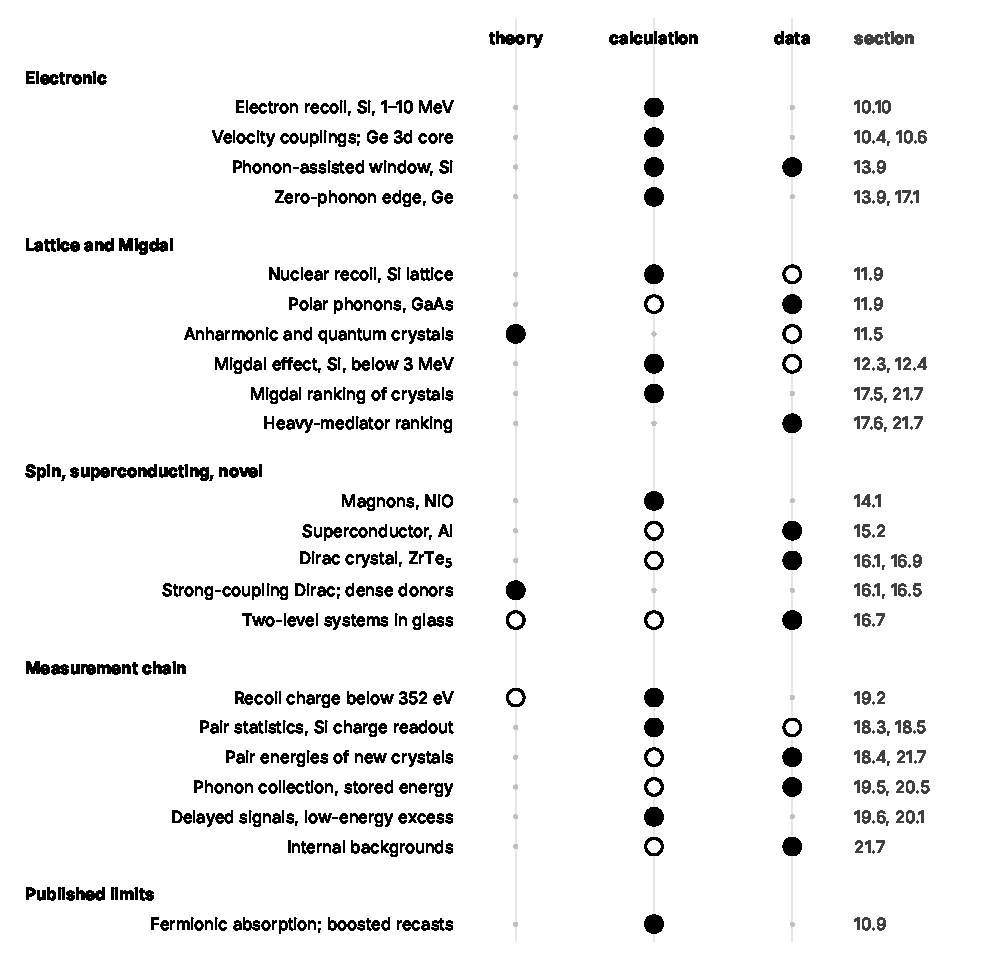
\includegraphics[width=0.92\linewidth]{figures/ch22/fig22_1.pdf}
  \caption{Channels of the book by the factor that limits them. Theory: no controlled approximation at the values the inputs take. Calculation: the next term has a known form and is computable, but is not computed for the material. Data: the response is in hand and the rate is as uncertain as a measured property of the sample. Filled circles mark the class of the item that dominates the uncertainty of the channel at its reference point, open circles a class that contributes. The right column gives the section that states the items. The classes are read from the open problems and nuisance tables of each chapter and from \cref{tab:21-dominant}.}
  \label{fig:22-limits}
\end{figure}

Of the 22 channels in the figure, 12 are limited first by calculation, 9 by data and 2 by theory; the phonon-assisted window of silicon counts under both calculation and data. The first theory-limited row is that of strongly anharmonic and quantum crystals at detector temperatures, whose response is bounded only by the band of its exact moments (\cref{sec:11.5}). The second joins Dirac crystals at strong coupling and silicon doped near the Mott density, where no small parameter remains (\cref{sec:16.1,sec:16.5}). In both, the next step is a method, not a run. Theory also contributes to the recoil charge, where the exchange--correlation spread of the close-collision kernel has a known sign and no known size, and to glass targets, whose two-level systems interact through their strain fields, outside the standard tunneling model of independent systems (\cref{sec:16.7}).

The calculation-limited rows hold the leading electron-recoil and Migdal results of the running example: the silicon rate above \SI{1}{MeV}, the phonon-assisted window, the germanium edge, the Migdal rate below \SI{3}{MeV} and the Migdal ranking. The silicon lattice rate belongs here too, since its small band is the difference between computed and measured phonon frequencies. In these channels the framework is complete and the numbers are missing. The data-limited rows are of two kinds. Some are rankings in which computed inputs stand in for measured ones: the elastic tensor of TeO$_2$ for the heavy-mediator row and the pair energies of crystals outside the validated range for the threshold in quanta (\cref{sec:21.7}). Others are properties of a given sample or detector. The polar rate of GaAs rests on the measured ratio of Born charge to dielectric constant, and the background tensor of ZrTe$_5$ moves its reach by a factor 2.8 (\cref{we:16-band}). The gap and mean free path of an aluminum film, the parameters of the two-level systems of one film, the collection of a stated detector and the $^{210}$Pb and cosmogenic activities of a crystal are of the same kind. For these no calculation in this book substitutes for the measurement.

Four calculations each replace a factor of order ten or an unsized rate in a leading result: the phonon-assisted loss function of silicon with the zero-phonon rate on common bins, the coherent Migdal response of silicon below $2q_{\mathrm{BZ}}$, the loss functions of the survivors near their gaps, and the close-collision kernel. The second holds nearly all of the light-mass Migdal rate, the third gives the Migdal row of the guide a reading, and the fourth decides the charge of every silicon recoil below \SI{352}{eV}. Germanium bands that pass the valley-order and mass checks would open the zero-phonon window of germanium, the survivor with the lowest electron-recoil threshold mass. On the data side, five measurements move a leading result: the cold absorption edge of silicon near its threshold (\cref{sec:13.9-open}), the pair energy of germanium at millikelvin with its phonon collection calibrated separately, the elastic constants of TeO$_2$, the $^{210}$Pb activity of lead that can be grown into a crystal (\cref{tab:21-guide}), and the two-bias measurement that separates collection from stored energy (\cref{sec:19.5}). A tagged-recoil Migdal measurement in silicon would test the chain from the kick to the count.
